\documentclass[13pt,a4paper]{article}

\usepackage[MeX]{polski}
\usepackage[utf8]{inputenc}
\usepackage{graphicx}
\usepackage{wrapfig}
\usepackage{color}
\usepackage{xcolor}
\usepackage{amsmath}
\usepackage{amssymb}
\usepackage[inkscapelatex=false]{svg}
\usepackage{array, makecell}
\usepackage{mhchem}
\usepackage{tabularx}
\usepackage{svg}
\usepackage{braket}

\usepackage{listings}
\definecolor{commentsColor}{rgb}{0.497495, 0.497587, 0.497464}
\definecolor{keywordsColor}{rgb}{0.000000, 0.000000, 0.635294}
\definecolor{stringColor}{rgb}{0.558215, 0.000000, 0.135316}
\definecolor{mygreen}{rgb}{0,0.6,0}
\definecolor{mygray}{rgb}{0.5,0.5,0.5}
\definecolor{mymauve}{rgb}{0.58,0,0.82}
\lstset{ %
    frame=single,
  backgroundcolor=\color{white},   % choose the background color
  basicstyle=\ttfamily\vspace{1em},
  breaklines=true,                 % automatic line breaking only at whitespace
  captionpos=b,                    % sets the caption-position to bottom
  commentstyle=\color{mygreen},    % comment style
  escapeinside={\%*}{*)},          % if you want to add LaTeX within your code
  keywordstyle=\color{blue},       % keyword style
  stringstyle=\color{mymauve},     % string literal style
}


\usepackage[T1]{fontenc}
\usepackage[utf8]{inputenc}
\usepackage[lf]{Baskervaldx} % lining figures
\usepackage[bigdelims,vvarbb]{newtxmath} % math italic letters from nimbus Roman
\usepackage[cal=boondoxo]{mathalfa} % mathcal from STIX, unslanted a bit
\renewcommand*\oldstylenums[1]{\textosf{#1}}

\usepackage{multicol}
\usepackage{colortbl}
\usepackage[Export]{adjustbox}
\adjustboxset{max size={0.9\linewidth}{0.9\paperheight}}
\usepackage[colorlinks=true,linkcolor=red,citecolor=green]{hyperref}

\textwidth=16cm
\textheight=23cm
\topmargin=-2cm
\oddsidemargin=0cm
\setlength{\parindent}{0em}
\setlength{\parskip}{0.6em}
\setlength{\jot}{12pt}
\renewcommand{\arraystretch}{1.4}
\renewcommand{\theadfont}{\bfseries}
\newcommand{\todo}[1]{\textcolor{red}{TODO: #1}}
\newcommand{\const}{\text{const}}


\begin{document}
\title{
	\LARGE
	\textbf{Rozprzestrzenianie się informacji w sieci\\ -  podsumowanie wyników}
}
\author{
	\large
	Dawid Karpiński, 26.05.2024 r.
}
\date{}
\maketitle


\section{Implementacja modelu.}

Jako model rozprzestrzeniania się informacji wykorzystano model SIS (Susceptible-Infected-Susceptible). W nim, każdy węzeł w sieci może znajdować się w jednym z dwóch stanów: podatny na informację (Susceptible) lub posiadający informację (Infected).

Węzły posiadające informację mogą przekazywać ją dalej swoim podatnym sąsiadom z ustalonym prawdopodobieństwem $\beta$, natomiast sam zarażony węzeł może zapomnieć informację z prawdopodobieństwem $\gamma$ i ponownie stać się podatny.

\begin{lstlisting}[language=go,caption={\centering\textbf{Fragment kodu symulacji napisanego w języku Go.\\Cały kod do projektu zamieszczono na \url{https://github.com/davkk/sis-model}.}},label={code:main}]
var sim Simulation
sim.parseConfig()
// ...
steps := int(1e3)
// ...
infected := 1
maxK := graph.Nodes[graph.MaxDegreeNode()].K
for step := 0; step < steps; step++ {
    for idx := 0; idx < sim.N; idx++ {
        node := &graph.Nodes[idx]
        if node.K > 0 && node.Value == Infected {
            for _, nnIdx := range graph.AdjList[idx] {
                nnNode := &graph.Nodes[nnIdx]
                if nnNode.Value == Infected {
                    continue
                }
                if rand.Float64() < sim.beta(node.K, maxK) {
                    nnNode.Value = Infected
                    infected++
                }
            }
            if rand.Float64() < sim.gamma(node.K, maxK) {
                node.Value = Susceptible
                infected--
            }
        }
    }
}
\end{lstlisting}

W symulacji (listing \ref{code:main}) zachodzą następujące operacje:
\begin{enumerate}
	\item Inicjalizacja parametrów symulacji.
	\item Iteracja po każdym węźle w sieci.
	      \begin{itemize}
		      \item Wybór węzła posiadającego informację.
		      \item Węzły z informacją mogą przekazywać ją swoim podatnym sąsiadom z prawdopodobieństwem $\beta$.
		      \item Węzły z informacją mogą również ją zapomnieć z prawdopodobieństwem $\gamma$ i stawają się wtedy ponownie podatne.
	      \end{itemize}
\end{enumerate}

Symulacje zostały wykonane głównie na sieciach Barabasi-Albert (BA), natomiast do porównania wykorzystano także sieć Erdos-Renyi (ER).


\section{Wpływ stopnia pierwszego zarażonego węzła.}

Zbadano jak różne strategie wyboru początkowego węzła wpływają na dynamikę procesu zarażania.

\begin{figure}[ht!]
	\centering
	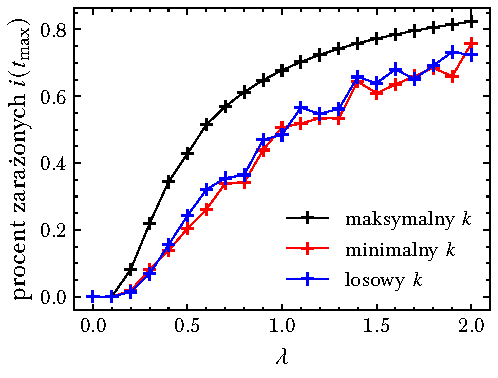
\includegraphics[width=\textwidth]{../figures/none/ba_max_min_rnd.pdf}
	\caption{\textbf{Porównanie pierwszego zarażonego o stopniu \boldmath{$k_{\min}$}, $\boldmath{k_{\max}}$ i losowym.}}
\end{figure}

Wykres ilustruje procent zarażonych węzłów $i(t_{\max})$ w funkcji współczynnika $\lambda=\frac{\beta}{\gamma}$ (stosunku wskaźnika przekazywania informacji do wskaźnika zapominania) dla trzech różnych strategii wyboru pierwszego zarażonego węzła.

\begin{itemize}
	\item Linia czarna ($k_{\max}$): Jak można zauważyć na wykresie, procent zarażonych węzłów rośnie najszybciej i osiąga najwyższe wartości przy danym $\lambda$
	\item Linia czerwona ($k_{\min}$): Procent zarażonych węzłów jest mniejszy w porównaniu z węzłem o maksymalnym stopniu, ale wciąż rośnie wraz ze wzrostem $\lambda$.
	\item Linia niebieska (losowy $k$): Wybór losowego węzła prowadzi do pośrednich wyników w porównaniu z dwoma pozostałymi strategiami. Procent zarażonych węzłów rośnie wolniej niż w przypadku węzła o maksymalnym $k$, ale szybciej niż w przypadku węzła o minimalnym $k$.
\end{itemize}

Zatem, początkowo zarażony węzeł o większej liczbie połączeń ma większy wpływ na rozprzestrzenianie się informacji, co jest zgodne z intuicją.

Warto zwrócić uwagę, że dla niskich wartości $\lambda$, różnice między strategiami wyboru pierwszego węzła są minimalne. Jednak w miarę wzrostu $\lambda$, różnice stają się bardziej wyraźne, wskazując na istotny wpływ wyboru strategii na efektywność rozprzestrzeniania się informacji.


\section{Modyfikacja parametrów.}

Poniżej zbadano wpływ różnych wartości parametrów modelu SIS na dynamikę rozprzestrzeniania się informacji w sieci. Dla każdego z przypadków ustalono $\gamma=0.1$ i zmieniano wartość $\beta$.

\subsection{$\boldmath{\beta,\gamma}=\const$}

Pierwszym przypadkiem jest klasyczny model, bez modyfikacji parametrów.

\begin{figure}[ht!]
	\centering
	\begin{minipage}[t]{0.49\textwidth}
		\centering
		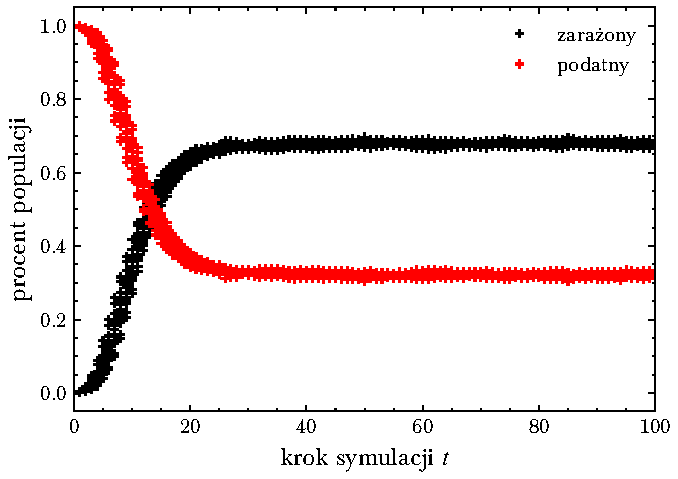
\includegraphics[width=\textwidth]{../figures/none/ba_infected_vs_step.pdf}
	\end{minipage}
	\begin{minipage}[t]{0.49\textwidth}
		\centering
		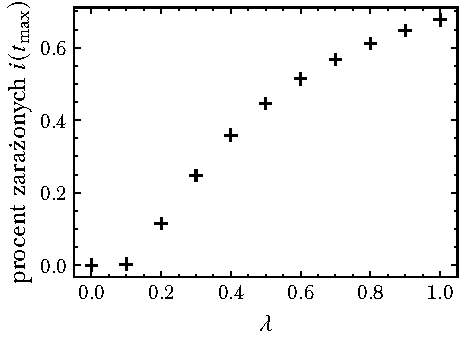
\includegraphics[width=\textwidth]{../figures/none/ba_infected_vs_ratio.pdf}
	\end{minipage}
	\caption{\centering\textbf{Przykładowy przebieg symulacji dla wybranych parametrów \boldmath{$\beta=0.1$}, $\gamma=0.1$ (lewo) i diagram fazowy $i_{\max}(\lambda)$ (prawo) dla BA, n=1000, m=2. Każdy punkt jest wynikiem uśrednienia 10 symulacji.}}
\end{figure}

Na początku przebiegu symulacji procent zarażonych szybko rośnie, osiągając maksimum, a następnie stabilizuje się na pewnej wartości. Natomiast, w miarę wzrostu $\lambda$, maksymalny procent zarażonych węzłów rośnie, co wskazuje na większą efektywność rozprzestrzeniania się informacji przy wyższym stosunku $\beta$ do $\gamma$.

\pagebreak

\begin{figure}[ht!]
	\begin{minipage}[t]{0.49\textwidth}
		\centering
		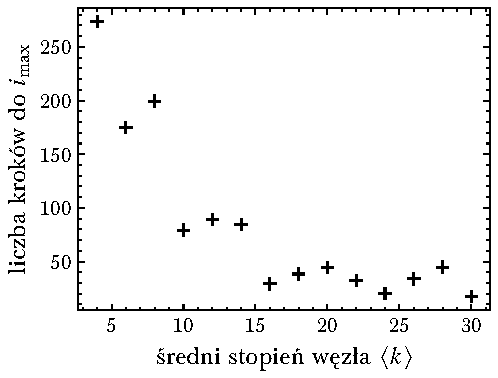
\includegraphics[width=\textwidth]{../figures/none/ba_tmax_vs_k.pdf}
	\end{minipage}
	\hspace{\fill}
	\begin{minipage}[t]{0.49\textwidth}
		\centering
		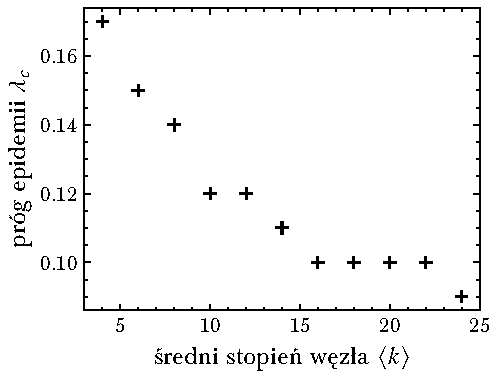
\includegraphics[width=\textwidth]{../figures/none/ba_threshold_vs_k.pdf}
	\end{minipage}
	\caption{\centering\textbf{Zależność liczby kroków do maksymalnej liczby zarażonych (lewo) i progu epidemii (prawo) od średniego stopnia węzła dla sieci BA, \boldmath{$n=1000$}. Każdy punkt jest wynikiem uśrednienia 10 symulacji.}}
\end{figure}

W miarę wzrostu średniego stopnia węzła, czas do osiągnięcia maksymalnej liczby zarażonych maleje, co sugeruje, że sieci o wyższym średnim stopniu węzła szybciej rozprzestrzeniają informacje.

Z kolei wartość $\lambda_c$ maleje wraz ze wzrostem średniego stopnia węzła, co oznacza, że w sieciach o wyższym średnim stopniu łatwiej dochodzi do rozprzestrzeniania się informacji (niższy próg $\lambda$).


\subsection{\texorpdfstring{\boldmath{$\beta \propto k$}}{beta proportional to k}, $\gamma=\const$}

Jako pierwszą modyfikację, wprowadzono do modelu zależność prawdopodobieństwa zarażenia $\beta$ od stopnia rozważanego węzła: $\beta(k_i)=\beta_0 \cdot k_i / k_{\max}$. W ten sposób ten parametr staje się indywidualny dla każdego węzła.

Zatem, im dany węzeł ma więcej połączeń, tym łatwiej przekaże informację dalej oraz łatwiej tę informację porzuci.

\begin{figure}[ht!]
	\begin{minipage}[t]{0.49\textwidth}
		\centering
		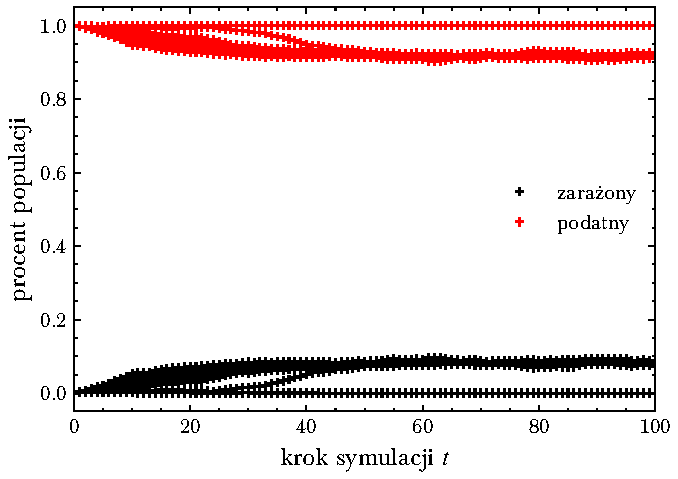
\includegraphics[width=\textwidth]{../figures/beta/ba_infected_vs_step.pdf}
	\end{minipage}
	\hspace{\fill}
	\begin{minipage}[t]{0.49\textwidth}
		\centering
		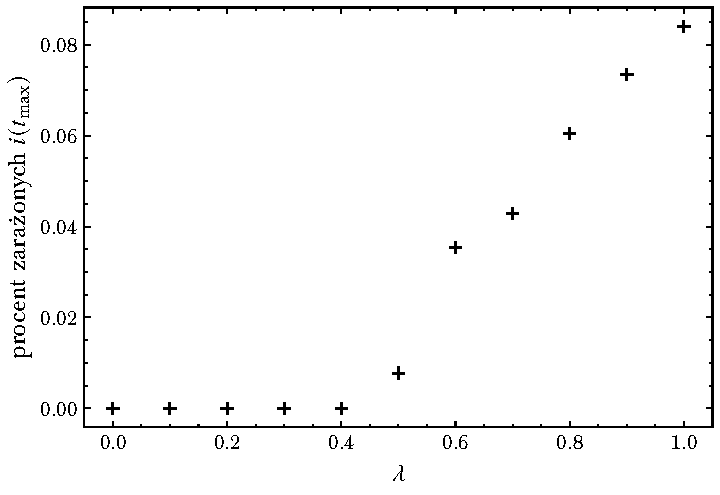
\includegraphics[width=\textwidth]{../figures/beta/ba_infected_vs_ratio.pdf}
	\end{minipage}
	\caption{\centering\textbf{Przykładowy przebieg symulacji dla wybranych parametrów \boldmath{$\beta=0.1$}, $\gamma=0.1$ (lewo) i diagram fazowy $i_{\max}(\lambda)$ (prawo) dla BA, n=1000, m=2. Każdy punkt jest wynikiem uśrednienia 10 symulacji.}}
\end{figure}

\pagebreak

Próg epidemii dla tego przypadku przesunął się w prawo względem wyniku dla klasycznego modelu. Wzrost procentu zarażonych również jest bardziej stromy.

\begin{figure}[ht!]
	\begin{minipage}[t]{0.49\textwidth}
		\centering
		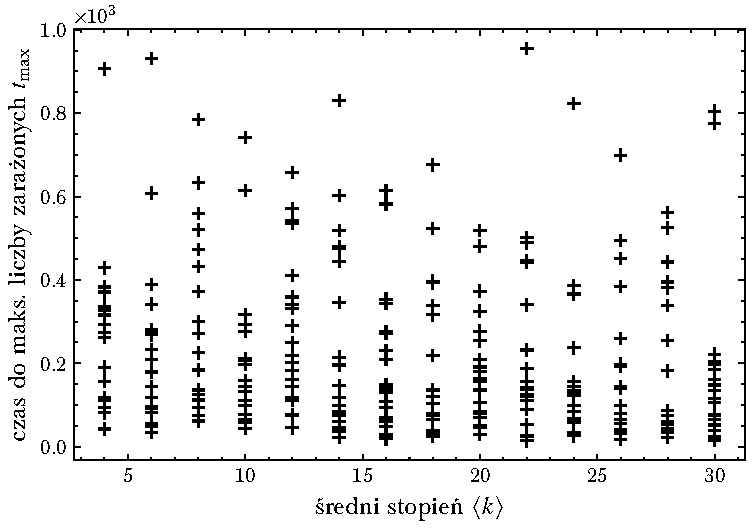
\includegraphics[width=\textwidth]{../figures/beta/ba_tmax_vs_k.pdf}
	\end{minipage}
	\hspace{\fill}
	\begin{minipage}[t]{0.49\textwidth}
		\centering
		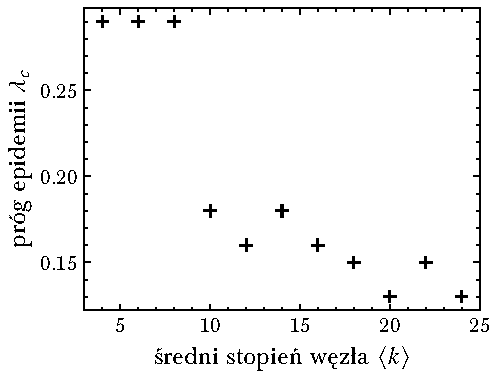
\includegraphics[width=\textwidth]{../figures/beta/ba_threshold_vs_k.pdf}
	\end{minipage}
	\caption{\centering\textbf{Zależność liczby kroków do maksymalnej liczby zarażonych (lewo) i progu epidemii (prawo) od średniego stopnia węzła dla sieci BA, \boldmath{$n=1000$}. Każdy punkt jest wynikiem uśrednienia 10 symulacji.}}
\end{figure}

Oba przebiegi od średniego stopnia zachowały swój trend (malejący), natomiast stały się mniej deterministyczne.


\subsection{$\boldmath{\beta=\const}$, \texorpdfstring{\boldmath{$\gamma \propto k$}}{gamma proportional to k}}

Następnie, analogicznie do przypadku wyżej, rozpatrzono przypadek gdzie to $\gamma$ zależy od stopnia węzła, a parametr $\beta$ jest stały.

\begin{figure}[ht!]
	\begin{minipage}[t]{0.49\textwidth}
		\centering
		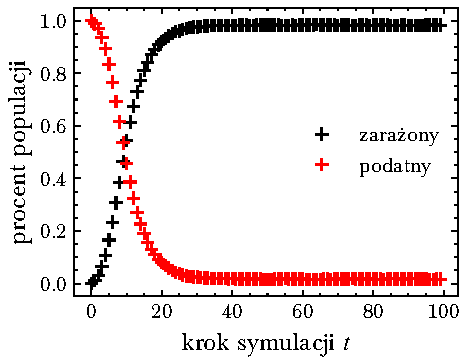
\includegraphics[width=\textwidth]{../figures/gamma/ba_infected_vs_step.pdf}
	\end{minipage}
	\hspace{\fill}
	\begin{minipage}[t]{0.49\textwidth}
		\centering
		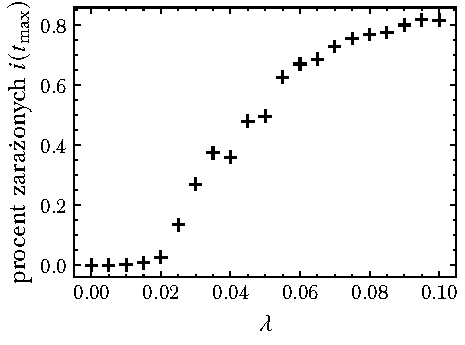
\includegraphics[width=\textwidth]{../figures/gamma/ba_infected_vs_ratio.pdf}
	\end{minipage}
	\caption{\centering\textbf{Przykładowy przebieg symulacji dla wybranych parametrów \boldmath{$\beta=0.1$}, $\gamma=0.1$ (lewo) i diagram fazowy $i_{\max}(\lambda)$ (prawo) dla BA, n=1000, m=2. Każdy punkt jest wynikiem uśrednienia 10 symulacji.}}
\end{figure}

\begin{figure}[ht!]
	\begin{minipage}[t]{0.49\textwidth}
		\centering
		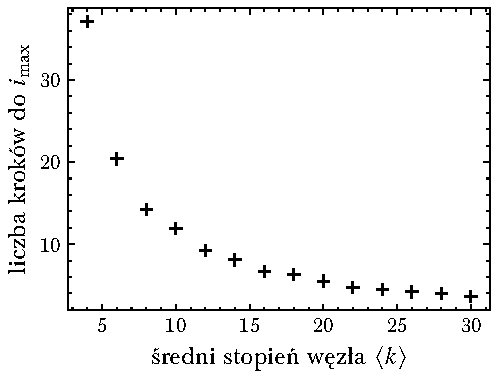
\includegraphics[width=\textwidth]{../figures/gamma/ba_tmax_vs_k.pdf}
	\end{minipage}
	\hspace{\fill}
	\begin{minipage}[t]{0.49\textwidth}
		\centering
		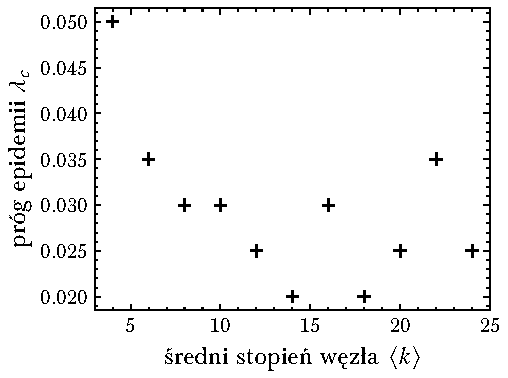
\includegraphics[width=\textwidth]{../figures/gamma/ba_threshold_vs_k.pdf}
	\end{minipage}
	\caption{\centering\textbf{Zależność liczby kroków do maksymalnej liczby zarażonych (lewo) i progu epidemii (prawo) od średniego stopnia węzła dla sieci BA, \boldmath{$n=1000$}. Każdy punkt jest wynikiem uśrednienia 10 symulacji.}}
\end{figure}
\pagebreak

Otrzymane wyniki wskazują, że zależność $\gamma=\gamma(k)$ powoduje skrócenie czasu przebiegu informacji i szybsze jej wygaszenie w sieci.


\subsection{\texorpdfstring{\boldmath{$\beta,\gamma \propto k$}}{beta and gamma proportional to k}}

Jako ostatni przypadek, zbadano model, w którym oba parametry zależą od stopnia węzła.

\begin{figure}[ht!]
	\begin{minipage}[t]{0.49\textwidth}
		\centering
		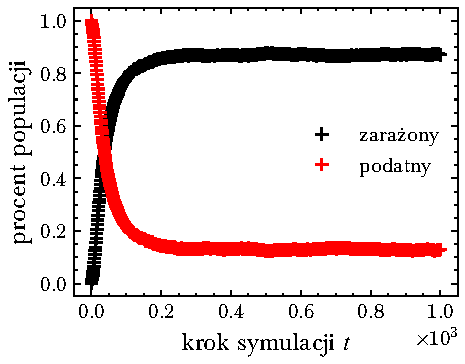
\includegraphics[width=\textwidth]{../figures/both/ba_infected_vs_step.pdf}
	\end{minipage}
	\hspace{\fill}
	\begin{minipage}[t]{0.49\textwidth}
		\centering
		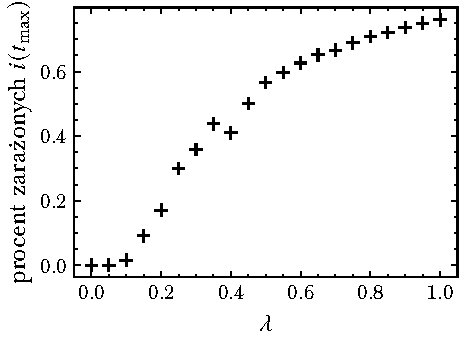
\includegraphics[width=\textwidth]{../figures/both/ba_infected_vs_ratio.pdf}
	\end{minipage}
	\caption{\centering\textbf{Przykładowy przebieg symulacji dla wybranych parametrów \boldmath{$\beta=0.1$}, $\gamma=0.1$ (lewo) i diagram fazowy $i_{\max}(\lambda)$ (prawo) dla BA, n=1000, m=2. Każdy punkt jest wynikiem uśrednienia 10 symulacji.}}
\end{figure}
\pagebreak

\begin{figure}[ht!]
	\begin{minipage}[t]{0.49\textwidth}
		\centering
		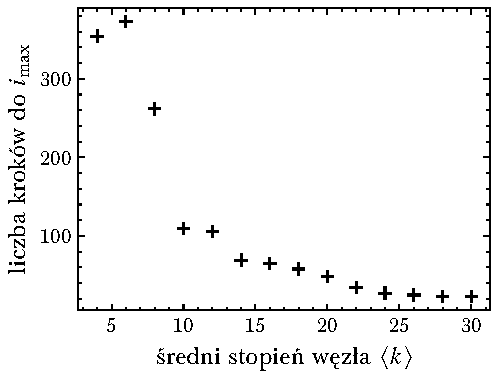
\includegraphics[width=\textwidth]{../figures/both/ba_tmax_vs_k.pdf}
	\end{minipage}
	\hspace{\fill}
	\begin{minipage}[t]{0.49\textwidth}
		\centering
		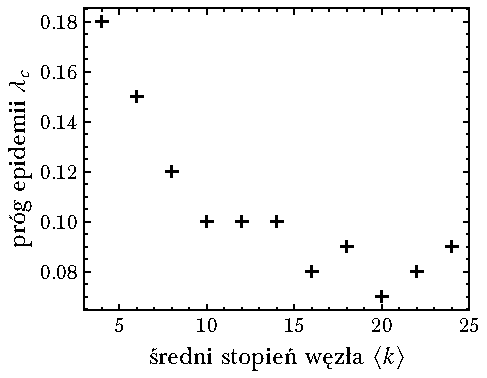
\includegraphics[width=\textwidth]{../figures/both/ba_threshold_vs_k.pdf}
	\end{minipage}
	\caption{\centering\textbf{Zależność liczby kroków do maksymalnej liczby zarażonych (lewo) i progu epidemii (prawo) od średniego stopnia węzła dla sieci BA, \boldmath{$n=1000$}. Każdy punkt jest wynikiem uśrednienia 10 symulacji.}}
\end{figure}

Symulacja modelu z obydwoma zmodyfikowanymi parametrami jest lekko wydłużona w stosunku do przypadku klasycznego. Niemniej jednak, poza tą różnicą zachowanie modelu jest zbliżone. Sugeruje to, że wpływ obu modyfikacji zależności od stopnia węzła się znosi, co prowadzi do podobnej dynamiki rozprzestrzeniania się informacji.


\end{document}
